% This will be the main document for the Social Networks paper to
% be written by the Eggnet team of Jordan Ell, Triet Huynh and Braden
% Simpson in association with Adrian Schroeter and Daniela Damian.
\documentclass[conference]{IEEEtran}
\usepackage{graphicx}

% Correct bad hyphenation here
\hyphenation{op-tical net-works semi-conduc-tor}

% Begin the paper here
\begin{document}


% Paper title
% Can use linebreaks \\ within to get better formatting as desired
\title{Changeset Based Communication to Detect Software Failures}

% Authors names
\author{\IEEEauthorblockN{Jordan Ell,
Triet Huynh,
Braden Simpson, 
Adrian Schr{\"o}ter and
Daniela Damian}
\IEEEauthorblockA{University of Victoria,
Victoria, British Columbia\\\{jell, infiro, braden\}@uvic.ca, schadr@acm.org, danielad@cs.uvic.ca}
%\IEEEauthorblockA{\IEEEauthorrefmark{2}University of Victoria\\
%Victoria, British Columbia\\ infiro@uvic.ca}
%\IEEEauthorblockA{\IEEEauthorrefmark{3}University of Victoria\\
%Victoria, British Columbia\\ braden@uvic.ca}
%\IEEEauthorblockA{\IEEEauthorrefmark{4}University of Victoria\\
%Victoria, British Columbia\\ schadr@uvic.ca}
%\IEEEauthorblockA{\IEEEauthorrefmark{5}University of Victoria\\
%Victoria, British Columbia\\ danielad@cs.uvic.ca}}
}
% make the title area
\maketitle


% talk about networks. 
\begin{abstract}
As software systems get more complex, the companies developing them consist of larger teams and therefore resulting in more complex communication artifacts.  As these software systems grow, so does the impact of every action to the product.  To find out how to prevent software failure created by this growth and complexity, companies need to find out more efficient and effective ways to communicate.  This paper provides an analysis of communications artifacts, linked to changesets by using multiple methods of textual analysis on the artifact, as well as the changeset.  These methods results in analysis of these communication artifacts and their participants to produce a historical representation in the form of social networks, which can be used to detect software failures based on participants and communication.
\end{abstract}

\section{Introduction}

% Setup problem
Software failure is a bigger, more prevalent problem now than ever.  These failures can be catastrophic, causing billions of lost dollars, or even lives.  The main cause of these software failures are larger companies and products and their inherent complexity, causing the difficulty of developing high quality products to greatly increase.  One tactic employed to ease this difficulty is to make use of powerful collaborative development environments (CDE) such as (BugZilla\footnote{http://bugzilla.org}, Jira\footnote{http://atlassian.com/software/jira/overview}, RTC\footnote{http://www-01.ibm.com/software/rational/products/rtc/}, etc.).  These systems provide bug reports and other communication artifacts, the core components implementing a software product during development.  The importance of these components has been researched by Wolf et al\cite{4721184}.  The impact of these communication artifacts on the project is significant, and improving the impact or life-cycle of these communication artifacts is greatly desired.  Using social networks based on changesets, we study the participants and resultant snapshot of the project at that changeset to determine if there are any potentially harmful patterns of communication present.  

% Other research 
Other researchers such as Bettenburg et al\cite{Bettenburg:2008:ESI:1370750.1370757}. have done work to link communication artifacts to source code.  As well Sliwerski et al\cite{Sliwerski:2005:CIF:1083142.1083147}. have tried to link fixes(changesets) to their corresponding bug reports.  These studies can assist us to understand the direct impact of the communication, and all the effected artifacts.  

% Question
When companies make use of a CDE, over time, there emerges patterns of communication that can be observed, and actioned upon.  These patterns are a result of the people involved in the communication artifacts at the given changeset.   This causes us to ask the question: \textit{"Are there harmful communication patterns in social networks based on changesets and communications artifacts?"}  

% Method
This paper details our attempt at finding social networks at a changeset, and evaluating if any potentially harmful communication patterns can be detected.  These networks are useful for finding the potentially harmful patterns such as certain problematic groups of participants, or problem areas of a project that require more communication that another due to a more complex technical background. 

\section{Methodology}
Our goal is to detect potentially harmful patterns in social networks, and in the following sections we describe our methods used to detect these patterns by examining changeset based social networks.

\subsection{Linking CDE Data to Changesets}
Our goal here is to isolate all the communication artifacts that are involved in each changeset.  First, we attempt to link by checking the changeset comment for communication related identifiers, usually unique to the specific project.   When a strict match to this identifier is found, we construct a link between this changeset and the resulting issue(bug).  We consider this link to be of weight \textit{1.0}, out of our weighting scale from \textit{0.0 - 1.0}.  

\begin{figure}[h!]
\centering
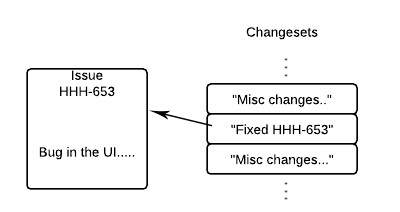
\includegraphics[width=1.0\columnwidth]{CommitsToChangesets}
\caption{The unique issue identifier found in a changeset comment.\label{fig:identifier}}
\end{figure}

After all the changeset comments have been parsed, we then attempt another method to link the communication to source files, at a certain date-range in the repository based on the date of the communication.  We accomplish this by parsing the communications artifacts for \textit{Stacktraces, Patches}, and \textit{Code Snippets} using similar methods as Bettenburg et al.\cite{Bettenburg:2008:ESI:1370750.1370757}.  We create confidence of each link based on the percentage of matched content, and stop at a threshold of 30 percent.  Once the links to files are created, we then check over a date range of X days around the time of the communication artifact for changesets that alter those files, and construct a link when one exists.  The weight of these links is calculated by the ratio of files referenced in the artifact to files matched in the changeset.

\begin{figure}[hb!]
\centering
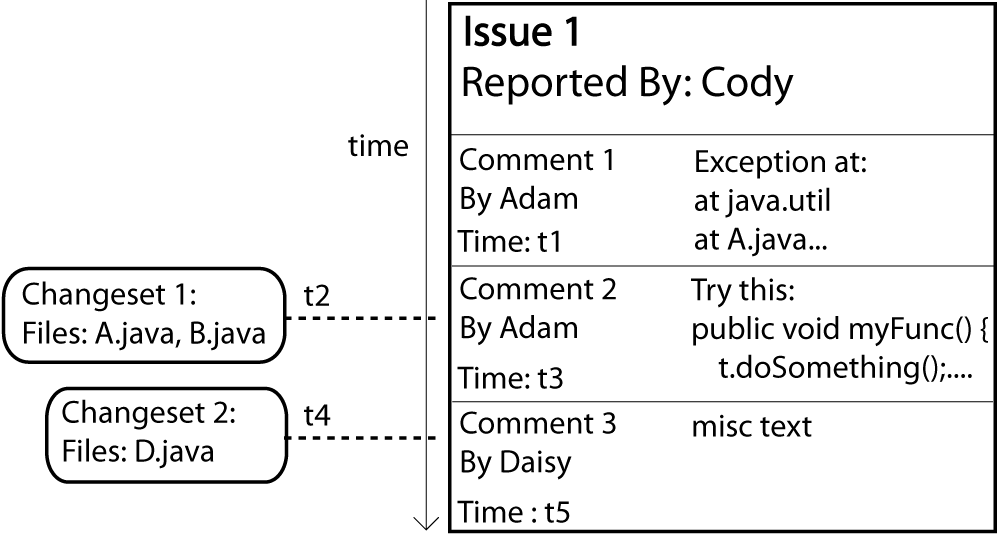
\includegraphics[width=1.0\columnwidth]{Items}
\caption{Timeline of issue, comments and changesets.\label{fig:items}}
\end{figure}

In Fig. 2, for example, there are links created between \emph{Changeset 1} and \emph{Comment 1}, since there is a \emph{Stacktrace} in \emph{Comment 1} that contains a match to the filename \emph{'A.java'} in \emph{Changeset 1}.  This will create a link between these artifacts and changesets, allowing us to determine the impact of the social network created by these communication artifacts surrounding a changeset.

\subsection{Creating Social Networks} 
To create the social networks for a commit, we get all the linked communication to a changeset.   and then constuct what we call a \emph{thread}

\subsection{Determine Fix-Inducing Changes}
We qualify each commit as either a pass or fail, pass meaning that it was a commit that did not introduce a bug, and conversely a fail is a commit that introduced a bug.  The method used to calculate this was derived from Sliwerski et al.\cite{Sliwerski:2005:CIF:1083142.1083147}. 

\subsection{Social Network Analysis}
The next step is to construct networks of communication between participants of the communications artifacts for each changeset.  Then, based on these per-changeset networks, analyze the patterns created and calculate our measures such as .  Some of these being based on these links, making 

\section{Results}
\subsection{Data Collection}
We used Hibernate-ORM\footnote{An open source Java library that is used for creating object-relational mappings for data-modeling} as a case study.  It is hosted on GitHub, and managed by Jira\footnotemark[2].  Our project requires that both the repository information and the CDE data is able to be mined in order to create the social networks.

\subsection{Rest}
todo figure out title of this section

\section{Conclusion and Future Work}
Describe our conclusion.


\section*{Acknowledgment}
The authors would like to thank yo' mama.


\bibliographystyle{IEEEtran}
\bibliography{paper}

% End of the paper
\end{document}

